%========================= Classe du Document ==========================
\documentclass[a4paper,fleqn]{article}
%============================= Packages ================================
\usepackage[margin=2.5cm]{geometry}
\usepackage[hidelinks]{hyperref}
\usepackage[utf8]{inputenc}
\usepackage[T1]{fontenc}
\usepackage{graphicx}
\usepackage{listings}
\usepackage{amsmath}
\usepackage{amsfonts}
\usepackage{amssymb}
\usepackage[version=4]{mhchem}
\usepackage{stmaryrd}
\usepackage{graphicx}
\usepackage{footmisc}
\usepackage{amssymb}
\usepackage{hyperref}
\usepackage{xcolor}
\usepackage{algorithm}
\usepackage{algpseudocode}
\usepackage{listings}
\usepackage{afterpage}
    
\definecolor{codegreen}{rgb}{0,0.6,0}
\definecolor{codegray}{rgb}{0.5,0.5,0.5}
\definecolor{codepurple}{rgb}{0.58,0,0.82}
\definecolor{backcolour}{rgb}{0.95,0.95,0.92}


\lstdefinestyle{mystyle}{
    backgroundcolor=\color{backcolour},   
    commentstyle=\color{codegreen},
    keywordstyle=\color{magenta},
    numberstyle=\tiny\color{codegray},
    stringstyle=\color{codepurple},
    basicstyle=\ttfamily\footnotesize,
    breakatwhitespace=false,         
    breaklines=true,                 
    captionpos=b,                    
    keepspaces=true,                 
    numbers=left,                    
    numbersep=5pt,                  
    showspaces=false,                
    showstringspaces=false,
    showtabs=false,                  
    tabsize=2
}

\lstset{style=mystyle}
\usepackage[french]{babel}
\setlength{\parindent}{0pt}
%=======================================================================

\parindent=1cm

%========================= Debut du document ===========================
\begin{document}
%=======================================================================


%^^^^^^^^^^^^^^^^^^^^^^^^^^^ Page de Garde ^^^^^^^^^^^^^^^^^^^^^^^^^^^^^
\definecolor{color}{HTML}{FFFFFF}
\pagecolor{color}
\thispagestyle{empty}

\begin{figure}
    \centering
    
\includegraphics[width=8cm]{./uspn.png}
\end{figure}

\vspace{6cm}

\begin{center}
    {\huge \bfseries Puissance 4 \par}
    
    \vspace{1cm}
    
    \begin{figure}[h]
        \centering
        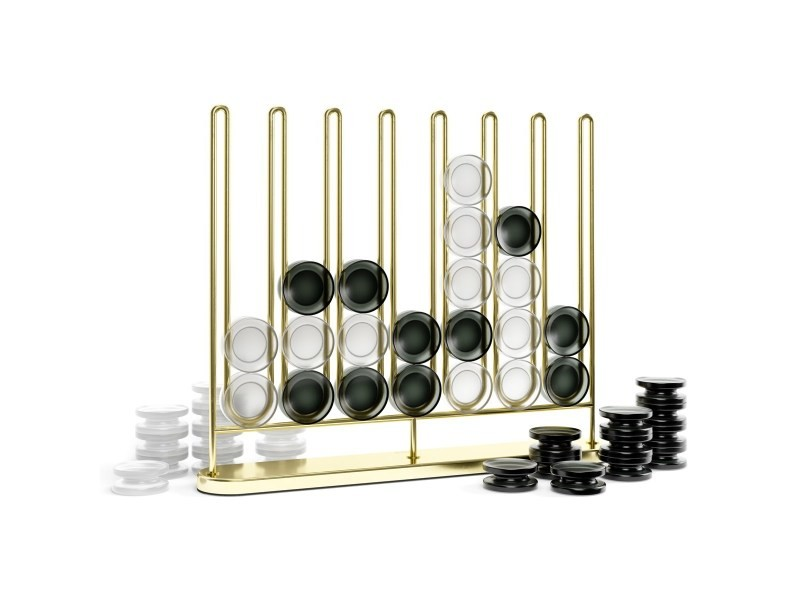
\includegraphics[width=8cm]{./cover.jpeg}
    \end{figure}
    
    \vspace{2cm}
    
    \large Structures de Données - J.CHAUSSARD \\
    
    \vspace{1cm}
    E.NICOLAS -- Y.BEN KAOUDJT\\
    \vspace{0.3cm}
    ING1 INFO - SUP GALILÉE \\
    \vspace{0.3cm}
    ethan.bento-nicolas@edu.univ-paris13.fr\\
    yanis.benkaoudjt@edu.univ-paris13.fr
    
    \vfill
   
    
    \today 
\end{center}
%^^^^^^^^^^^^^^^^^^^^^^^^^ Fin Page de Garde ^^^^^^^^^^^^^^^^^^^^^^^^^^
 
 \pagebreak
 
  ~
  
 \pagebreak
 
 \section*{Engagement de non-plagiat}

\vspace{0.5cm}
Nous, soussignés E.NICOLAS et Y.BEN KAOUDJT, étudiants en 1ère année d'école d'ingénieur à Sup Galilée,
déclarons être pleinement conscients que la copie de tout ou partie d'un document, quel qu'il
soit, publié sur tout support existant, y compris sur Internet, constitue une violation du droit
d'auteur ainsi qu'une fraude caractérisée, tout comme l’utilisation d’outils d’Intelligence
Artificielle pour générer une partie de ce rapport ou du code associé.
En conséquence, nous déclarons que ce travail ne comporte aucun plagiat, et assurons avoir cité
explicitement, à chaque fois que nous en avons fait usage, toutes les sources utilisées pour le
rédiger.\\

\hspace{9.7cm}Fait à Villetaneuse, le 26/01/2024\\

\hspace{13cm}E.N -- Y.BK

\begin{figure}[h]
        \centering
     
    \end{figure}

\pagebreak

\tableofcontents
\vspace{1cm}
\lstlistoflistings

\pagebreak

\section{Introduction}

\subsection{Préface}

Actuellement en première année d'école d'ingénieur en spécialité informatique, et dans le cadre du cours de structure de données, nous avons eu l'occasion de pouvoir coder en C un jeu de Puissance 4. Celui-ci étant jouable en local a deux ou contre un ordinateur dopé a l'IA (algorithme MiniMax). L'interface de jeu proposée sera dans le terminal et il sera jouable avec un pavé numérique.

\subsection{Présentation des objectifs}

On souhaite élaborer un algorithme \textit{MiniMax} pour résoudre une partie de Puissance 4. Pour cela, l'algorithme choisis le coup optimal en calculant les "scores" des prochains coups (5 dans ce projet mais le paramètre peut être changé par une autre profondeur impaire, en effet le dernier coup dans MiniMax doit être joué par l'IA). Dans une première partie, nous verrons comment nous avons implémenté le jeu multijoueur en local et les difficultés que nous avons rencontrés. Dans une deuxième partie, nous discuterons plus en détail de l'algorithme MiniMax et verrons comment le construire et l'améliorer à l'aide de l'\textit{"AlphaBeta pruning"}. De plus, nous parlerons des structures utilisées et des algorithmes.

\section{Compilation et exécution du programme}

\begin{enumerate}
\item Ouvrir un terminal

\item Se placer dans le dossier contenant les fichiers sources puis entrer "make"

\item Lancer le programme avec "./puissance4.exe"

\item Suivre les instructions affichées

\item Après avoir quitté le jeu, si vous souhaitez supprimer l'exécutable, "make clean"
\end{enumerate}

\pagebreak

\section{Implémentation de la partie "Multijoueur local"}

\subsection{Prérequis}
 
On commence par définir comment représenter la grille de jeu.. Ainsi, pour représenter l'état de la partie : un tableau de X LIGNES et Y COLONNES (que l'on peut changer dans le fichier "puissance4.h") contenant des jetons sous forme d'entier. Ces jetons sont également définis dans ce fichier.
On utilise aussi des séquences d'échappement ANSI pour colorer les jetons dans le terminal \footnote{\url{https://gist.github.com/JBlond/2fea43a3049b38287e5e9cefc87b2124}}.\\

\begin{lstlisting}[language=C, caption=Représentation du puissance 4 et constantes en C]
// Extrait de puissance4.h
...
// Taille du plateau
#define LIGNES 6
#define COLONNES 7

// Jetons
#define JOUEUR1 1
#define JOUEUR2 2
#define IA 2

// Couleurs ANSI
#define DEFAUT "\e[0m"
#define ROUGE "\e[0;31m"
#define JAUNE "\e[0;33m"
#define VIOLET "\e[0;35m"
...

// Extrait de main.c
int main()
{    
	uint8_t plateau[LIGNES][COLONNES];
	...
}
\end{lstlisting}

\subsection{Prototypes des fonctions et logique}

Les fonctions sont rangés dans plusieurs fichiers selon leur utilisation. Il y a les fonctions d'affichage du menu et du plateau dans le fichier affichage.c. Les fonctions utiles au Puissance 4 local dans le fichier puissance4.c puis les fonctions de la deuxième partie dans noeud.c et minimax.c.\\

Pour le jeu en local nous avons besoin de fonctions pour placer un jeton dans une colonne, vérifier si la colonne n'est pas pleine, annuler un coup (utile dans la seconde partie), vérifier l'état de la partie (victoire ou égalité) et également une fonction "myscanf" qui gère les erreurs d'entrée. \\

Prototypage des fonctions \footnote{Voir le fichier puissance4.h} :

\begin{itemize}
\item Les fonctions d'affichage sont de la forme "void fonction()", sauf pour "afficherPlateau" à qui l'on passe une grille de jeu.
\item L'initialisation de la grille, la placement et l'enlèvement d'un jeton sont en void car elles ne servent pas a donner d'informations dans la boucle de jeu. Cependant, les autres fonctions sont toutes booléennes car elles sont utilisées dans des structures de contrôle. On passe en paramètres la grille, le jeton et/ou la colonne.
\end{itemize}
\vspace{0.5cm}

En ce qui concerne la logique, les fonctions du Puissance 4 en local sont assez triviales. La seule fonction qui ait posé quelques soucis est la vérification du gagnant en fonction du dernier coup joué. Il a fallu penser à toutes les configurations de victoire possibles.

Pour cela, on commence par récupérer la ligne du dernier coup joué en utilisant la colonne passé en paramètre. Ensuite, on découpe les 4 cas possibles, soit les quatre jetons sont : en ligne, en colonne, en diagonale ascendante ou descendante.

Pour cela, on imagine que le jeton est à n'importe quelle place de la suite et donc on fait une boucle qui vérifie pour chaque position. Avant d'accéder au cases du tableau, on vérifie que l'indice du premier et du dernier accès sont compris dans le tableau. On fait de même pour les colonnes.

Les diagonales suivent la même logique en ajoutant des conditions sur les indices en hauteur et en largeur et en modifiant les indices des lignes et des colonnes. Pour les descendantes c'est le même indice dans les deux et on fait la vérification de droite à gauche. Pour les ascendantes c'est pareil mais les indices des colonnes sont inversées par rapport aux descendantes, c'est à dire qu'on regarde de gauche à droite \footnote{Voir le fichier puissance4.c ligne 52}. Une fois la partie terminée par une victoire ou une égalité, on retourne dans le menu et l'on peut recommencer d'autres parties.

\pagebreak

\section{Implémentation de la partie "Solo"}

\subsection{Prérequis}

On commence par définir comment représenter un arbre ; une structure noeud possédant une grille de jeu, le joueur ayant joué le coup, la colonne de ce coup et une liste chainée d'enfants. \\

\begin{lstlisting}[language=C, caption=Représentation d'un noeud en C]
// Extrait de puissance4.h
...

// Profondeur de l'arbre pour l'algorithme minimax
#define PROFONDEUR 5

/typedef struct noeud
{
    uint8_t plateau[LIGNES][COLONNES];  // Grille de jeu
    uint8_t joueur;                    // Joueur ayant joue le coup associe au noeud
    uint8_t colonne;                  // Colonne jouee
    struct noeud *enfant;            // Liste chainee d'enfants
    struct noeud *suivant;          // Enfant suivant
} noeud;
...

\end{lstlisting}

\subsection{Discussion autour de l'algorithme MiniMax}

Afin de pouvoir jouer au puissance 4 en "solo", il était nécessaire d'implémenter un algorithme permettant à l'ordinateur de jouer, mais sans que celui-ci n'effectue que des coups au "hasard". Ainsi, l'idée de l'algorithme MiniMax est de parcourir l'arbre de possibilités de coups et d'évaluer ceux-ci. Ensuite, pour choisir le coup optimal, on maximise le score lors du tour de l'IA et on minimise lors du coup du joueur  En ce qui concerne la complexité, le MiniMax s'exécute en O($L^P$), avec L la largeur du plateau et P la profondeur de l'arbre des coups. Il est possible d'optimiser l'algorithme afin d'obtenir une meilleure complexité, c'est ici qu'intervient l'élagage Alpha-Bêta.

\subsection{Élagage Alpha-Bêta}

L'algorithme Alpha-Bêta est une optimisation de l'algorithme MiniMax. Le principe est de réaliser une exploration partielle plutôt que complète de l'arbre, car certains sous-arbres mènent à des configurations qui ne seront pas utilisées pour la remontée du score. Cela est possible dans l'hypothèse où la fonction d'évaluation du score est assez correcte. Cet ajout permet d'obtenir une meillleur complexité environ O($\sqrt{L^d}$) dans le meilleur des cas \footnote{\url{https://en.wikipedia.org/wiki/Alpha-beta_pruning}}.\\

L'algorithme Alpha-Bêta tire son appellation des paramètres "Alpha" et "Bêta", qui représentent respectivement les valeurs minimales pour l'IA (MAX) et les valeurs maximales pour le joueur (MIN). L'idée est que lors de la recherche, si une valeur dépasse le "Bêta" pour un nœud MIN, ou étant inférieure à l'"Alpha" pour un nœud MAX, on peut arrêter de regarder le score des autres enfants et remonter la valeur MAX ou MIN.\\

\pagebreak

\subsection{Création de l'arbre et application des scores dans la remontée}

\begin{lstlisting}[language=C, caption=Construction de l'arbre en C]

// Extrait de noeud.c
...
// Construire l'arbre des coups possibles avec leur score
void construireArbre(noeud *racine, uint8_t profondeur, uint8_t joueur, uint8_t adversaire, bool tourJoueur)
{
    if (profondeur == 0)
    {
        return;
    }

    for (uint8_t col = 0; col < COLONNES; col++)
    {
        if (!colonneEstPleine(racine->plateau, col))
        {
            placerJeton(racine->plateau, col, joueur);

            noeud *nouveauNoeud = creerNoeud(racine->plateau, col);

            if (tourJoueur)
                nouveauNoeud->joueur = joueur;
            else
                nouveauNoeud->joueur = adversaire;

            ajouterEnfant(racine, nouveauNoeud);

            if (!verifierGagnant(nouveauNoeud->plateau, joueur, col) && !verifierGagnant(nouveauNoeud->plateau, adversaire, col))
            {
                construireArbre(nouveauNoeud, profondeur - 1, adversaire, joueur, true ^ tourJoueur);
            }
            
            annulerCoup(racine->plateau, col);
        }
    }
}
...
\end{lstlisting}

Lors de la création d'un noeud, on recopie la grille passée en paramètre dans le plateau du noeud ainsi que la colonne et le joueur associé à cette grille .\\

L'ajout d'un enfant à a la liste chaînée se fait en prenant l' enfant passé en paramètre et en l'ajoutant à la pile d'enfants. On prends l'ancien enfant que le parent pointe et l'on le mets en tant que suivant du nouvel enfant puis on fait pointer le parent vers ce nouvel enfant.\\

La création récursive de l'arbre est assez simple, on a une condition d'arrêt donné par la profondeur souhaité et sinon on crée un noeud pour chaque colonne si c'est possible (colonne non-pleine), que l'on ajoute à l'arbre. On vérifie l'état du plateau de ce nouveau noeud pour éviter d'explorer si l'on a une victoire du joueur ou de l'adversaire. Pour savoir qui joue le coup, on passe en paramètre un booléen représentant le tour du joueur si vrai. Lors du rappel récursif à la fonction, on fait un XOR avec vrai pour savoir si c'est au tour de l'adversaire (ainsi "tourJoueur" est à "false" si c'est l'adversaire).

\pagebreak

\subsection{Implémentation du MiniMax avec élagage Alpha-Bêta et de l'heuristique d'évaluation}

Pour pouvoir garder les scores des 7 colonnes et les afficher, la fonction minimax qui renvoie le coup à jouer appelle une sous-fonction récursive "evaluerNoeud" qui s'occupe de remonter le score en utilisant l'algorithme MiniMax avec élagage Alpha-Bêta. La fonction renvoie le score du plateau lorsque la profondeur 0 est atteinte en partant de PROFONDEUR (défini à 5, voir la sous-section 3.1) puis remonte le score en maximisant ou en minimisant en remontant les appels de fonction. Ainsi, dans "minimax", pour les 7 premiers coups possibles on prends le meilleur. On peut aussi regarder si des scores sont égaux et prendre celui qui est le plus proche du centre (rien n'est indiqué dans l'énoncé sur ce sujet).\\

En ce qui concerne l'évaluation de la grille, on reprends la même logique que la fonction pour vérifier le gagnant, on passe dans chaque ligne chaque colonne et on passe les 4 cases à "evaluerSuite" qui donne le score en fonctions du nombres de jetons comme expliqué dans l'énoncé.\\

Fonctionnement du MiniMax avec Alpha-Bêta:  \\
\begin{itemize}

\item Lors du premier appel à la fonction "evaluerNoeud", on place Alpha à $-\infty$ (INT32MIN) et Bêta à $\infty$ (INT32MAX).\\

\item L'algorithme explore de manière récursive les nœuds de l'arbre et es valeurs Alpha et Bêta sont constamment actualisées en fonction des résultats obtenus au cours de l'exploration..\\

\item Lorsqu'une valeur est repérée dépassant le Bêta pour un nœud MAX ou étant inférieure à l'Alpha pour un nœud MIN, on interromps l'exploration de cette branche et on remonte le score. \\

\end{itemize}

\begin{lstlisting}[language=C, caption=Minimax utilisé avec élagage en C]

// Extrait de minimax.c
...
void minimax(uint8_t plateau[LIGNES][COLONNES], uint8_t *colonne, uint8_t joueur, uint8_t adversaire)
{
    noeud *racine = creerNoeud(plateau, 0);
    construireArbre(racine, PROFONDEUR, joueur, adversaire, true);

    int64_t meilleurScore = INT64_MIN;
    ...
    // Parcourir les enfant de la racine (les coups possibles)
    for (noeud *enfant = racine->enfant; enfant != NULL; enfant = enfant->suivant)
    {
        int64_t scoreEnfant = evaluerNoeud(enfant, PROFONDEUR, INT64_MIN, INT64_MAX, false, joueur, adversaire);
        ...
        if (scoreEnfant > meilleurScore)
        {
            meilleurScore = scoreEnfant;
            *colonne = enfant->colonne;
        }
     }
    ...
    libererArbre(racine);
}

// Fonction pour evaluer le score d'un noeud en utilisant l'algorithme minimax avec elagage alphabeta
int32_t evaluerNoeud(noeud *n, int32_t alpha, int32_t beta, bool maximiser, uint8_t joueur, uint8_t adversaire)
{
    if (n->enfant == NULL)
    {
        if (n->joueur == joueur)
            return score(n->plateau, joueur, adversaire);
        else if (n->joueur == adversaire)
            return score(n->plateau, adversaire, joueur);
    }

    // Si c'est le tour de l'IA (maximisation)
    if (maximiser)
    {
        int32_t score = INT32_MIN;

        for (noeud *enfant = n->enfant; enfant != NULL; enfant = enfant->suivant)
        {
            int32_t scoreEnfant = evaluerNoeud(enfant, alpha, beta, false, joueur, adversaire);
            score = max(score, scoreEnfant);

            if (score > beta)
                break;
            alpha = max(alpha, score);
        }

        return score;
    }
    // Si c'est le tour de l'humain (minimisation)
    else
    {
        int32_t score = INT32_MAX;

        for (noeud *enfant = n->enfant; enfant != NULL; enfant = enfant->suivant)
        {
            int32_t scoreEnfant = evaluerNoeud(enfant, alpha, beta, true, joueur, adversaire);
            score = min(score, scoreEnfant);

            if (score < alpha)
                break;
            beta = min(beta, score);
        }

        return score;
    }
}
...
\end{lstlisting}

L'algorithme utilisé en pseudo-code \footnote{\href{https://fr.wikipedia.org/wiki/\%C3\%89lagage_alpha-b\%C3\%AAta}{\nolinkurl{https://fr.wikipedia.org/wiki/Elagage_alpha-beta}}}:

\begin{lstlisting}[language=Pascal, mathescape=true, caption=Algorithme Alpha-Bêta en pseudo-code]
fonction alphabeta(noeud, $\alpha$, $\beta$) /* $\alpha$ est toujours inferieur a $\beta$ */
   si noeud est une feuille alors
       retourner la valeur de noeud
   sinon 
       si noeud est Min alors
           $v = \infty$
           pour tout fils de noeud faire
               $v = \min(v, \text{alphabeta}(fils, \alpha, \beta))$                
               si $\alpha \geq v$ alors  /* coupure alpha */
                   retourner $v$
               $\beta = \min(\beta, v)$           
       sinon
           $v = -\infty$
           pour tout fils de noeud faire
               $v = \max(v, \text{alphabeta}(fils, \alpha, \beta))$                
               si $v \geq \beta$ alors /* coupure beta */
                   retourner $v$
               $\alpha = \max(\alpha, v)$
   retourner $v$
\end{lstlisting}

\pagebreak

\section{Conclusion}

Après de nombreuses parties contre l'IA et en la faisant jouer contre d'autre IA sur internet on peut affirmer qu'elle joue assez bien. Perdu en 16 coups en jouant en deuxième contre un site ou le puissance 4 est résolu \footnote{\url{https://connect4.gamesolver.org/en/}}. On peut en conclure que le jeu est réussi même si on pourrait toujours faire mieux que ce soit dans la représentation des noeuds et de la gestion de la mémoire. Ce projet nous a permis de découvrir les algorithmes de jeux à somme nulle tel que MiniMax et d'Alpha-Bêta. Il ya aussi NegaMax ou le score est seulement l'opposé de l'autre, ou plus compliqué et se basant sur MCTS (Monte Carlo Tree Search) qui est la méthode heuristique implémenté dans AlphaGo (IA pour le jeu de go)\footnote{\url{https://fr.wikipedia.org/wiki/Recherche_arborescente_Monte-Carlo}}.\\

En somme, le projet à développé nos capacités d'analyse et de compréhension d'un sujet, mais nous a également permis d'augmenter notre curiosité sur les contours du sujet et ses implications. On a aussi pu travailler nos compétences en codage et en gestion de projet.\\

P.S : Pour un futur projet, le codage d'une deuxième méthode et la comparaison (temps de calculs, taux de victoire, espace occupé, ect.) entre les deux pourraient être intéréssante.\\

\hspace{6.5cm} FIN \newline

\pagebreak


\end{document}